\documentclass{article} 
\usepackage{color}
\usepackage{algorithmic}
\usepackage[small,bf]{caption}
\usepackage{float}
\usepackage{graphicx}

\graphicspath{{../}}

\floatstyle{plain}
\newfloat{program}{thp}{lop}
\floatname{program}{code}


\begin{document}
    
\title{Stock Exchange Server Simulator}
\author{Anton Morozov and Shubham Chopra}
\maketitle
    
\section{Introduction}

Observable processes such as car traffic or stock exchange are hard or impossible to predict yet we want to influence them. For instance, car traffic is observed using road sensors and can be controlled by street lights. Stock exchange is an observed stream of buy and sell requests that can be influenced by the additional trade requests. We want to influence these systems by creating algorithms to to improve control or to earn money. However making mistakes can be either costly or tragic. The algorithms are tested using the simulations of such systems before been applied to real applications. In simulations the historic data collected at some earlier date is augmented with new data produced by our algorithms to create variations of the original scenario. A set of user-defined rules specify how the historical and the new data interact to produce a coherent realistic stream of output events indistinguishable from real data stream. Our goal is to create a unified language for specifying simulations from historical data.

Each process can be thought of as a set of update streams to a set of relational tables. The simulator of the process will have the same set of update streams recorded at an earlier date (a historic data stream) and it will also have an additional set of update streams (a simulated data stream) coming from the algorithms being tested. The simulator combines them to produce a specified stream. 

%Our goal is to create a unified format for specifying simulations from historical data. In many instances it is hard, expensive or downright impossible to create a scenario similar to the one that produced the original historic data. Usually the simulations of such scenarios are created. In simulations the data from the original experiment is augmented with new data to create variations of the original scenario. A set of user defined rules specify how the historical and the new data interact to produce the desired outcome. Below we describe a format that allows us to specify those rules freely. 


\section{Approach}

At a high level, a historical data stream together with a simulated data streams can be thought of as update streams to a set of relational table. We assume that we have a set $S_i$ of $n$ update streams. Each of these streams can be filtered from in a set $S_f$ of $n$ filtered streams. Further the streams can be further combined or subdivided into a set $S_m$ of $k$ streams. For each in $S_m$ users provide a set of rules to produce the desired simulation outcomes. Those outcomes form a set $S_r$ of $k_r \geq k$ streams. The streams after rule application can again be combined into a set $S_m '$ of $t$ streams. The resultant streams are filtered before being returned to the users.
 
In this paper we will use a Stock Exchange simulator as an example. The simulators has two input streams. The first input stream is a stream of trade requests occurred at an earlier date. The second stream consists of trade requests coming from trading algorithms. The goal of the simulator is to incorporate this additional stream of trade requests to produce a realistic output stream might have occurred in a real stock exchange if the additional stock requests were given to it. Based on this simulator we will show how a similar simulator can be build. 

%In this paper we will be using a simulator for the stock exchange as an example. The goal of this simulator is to approximate an outcome of adding buy/sell stock request to a stream of stock exchange occurred at some earlier date. The stock exchange simulator can be thought of as a stream processor. There are $N$ incoming streams. Each of these streams is filtered to add or remove certain tuples. Later the streams are merged together if needed. After the merging step, the streams form $K$ order-book relations. Matching rules are applied to these on these relations. Matching rules form a set of output streams.

The process for creating a simulator is given in five steps:

\begin{enumerate}
    \item {\bf Input Filter}: Tuples are passed through a set of input filters, which can result in the removal or insertion of tuples. 
    \item {\bf Input Merging}: Each input stream after the filtering step can be split into several streams or be merged with other streams. We call this a merging step and it results in a set $S_m$ of $k$ streams. 
    \item {\bf Simulator Rules Application}: After a merging step each stream is materialized as a set of relations. These relations are reduced/matched using rules given by the user resulting in a set $S_r$ of streams.
    \item {\bf Output Merging}: The output merging step mirrors the input merging step. Here the streams again are combined or split into a set $S_M '$ of streams. 
    \item {\bf Output Filter}: Mirroring the input filter the output filter imposes additional transformations to the output tuples.
\end{enumerate}

%\begin{figure}
%  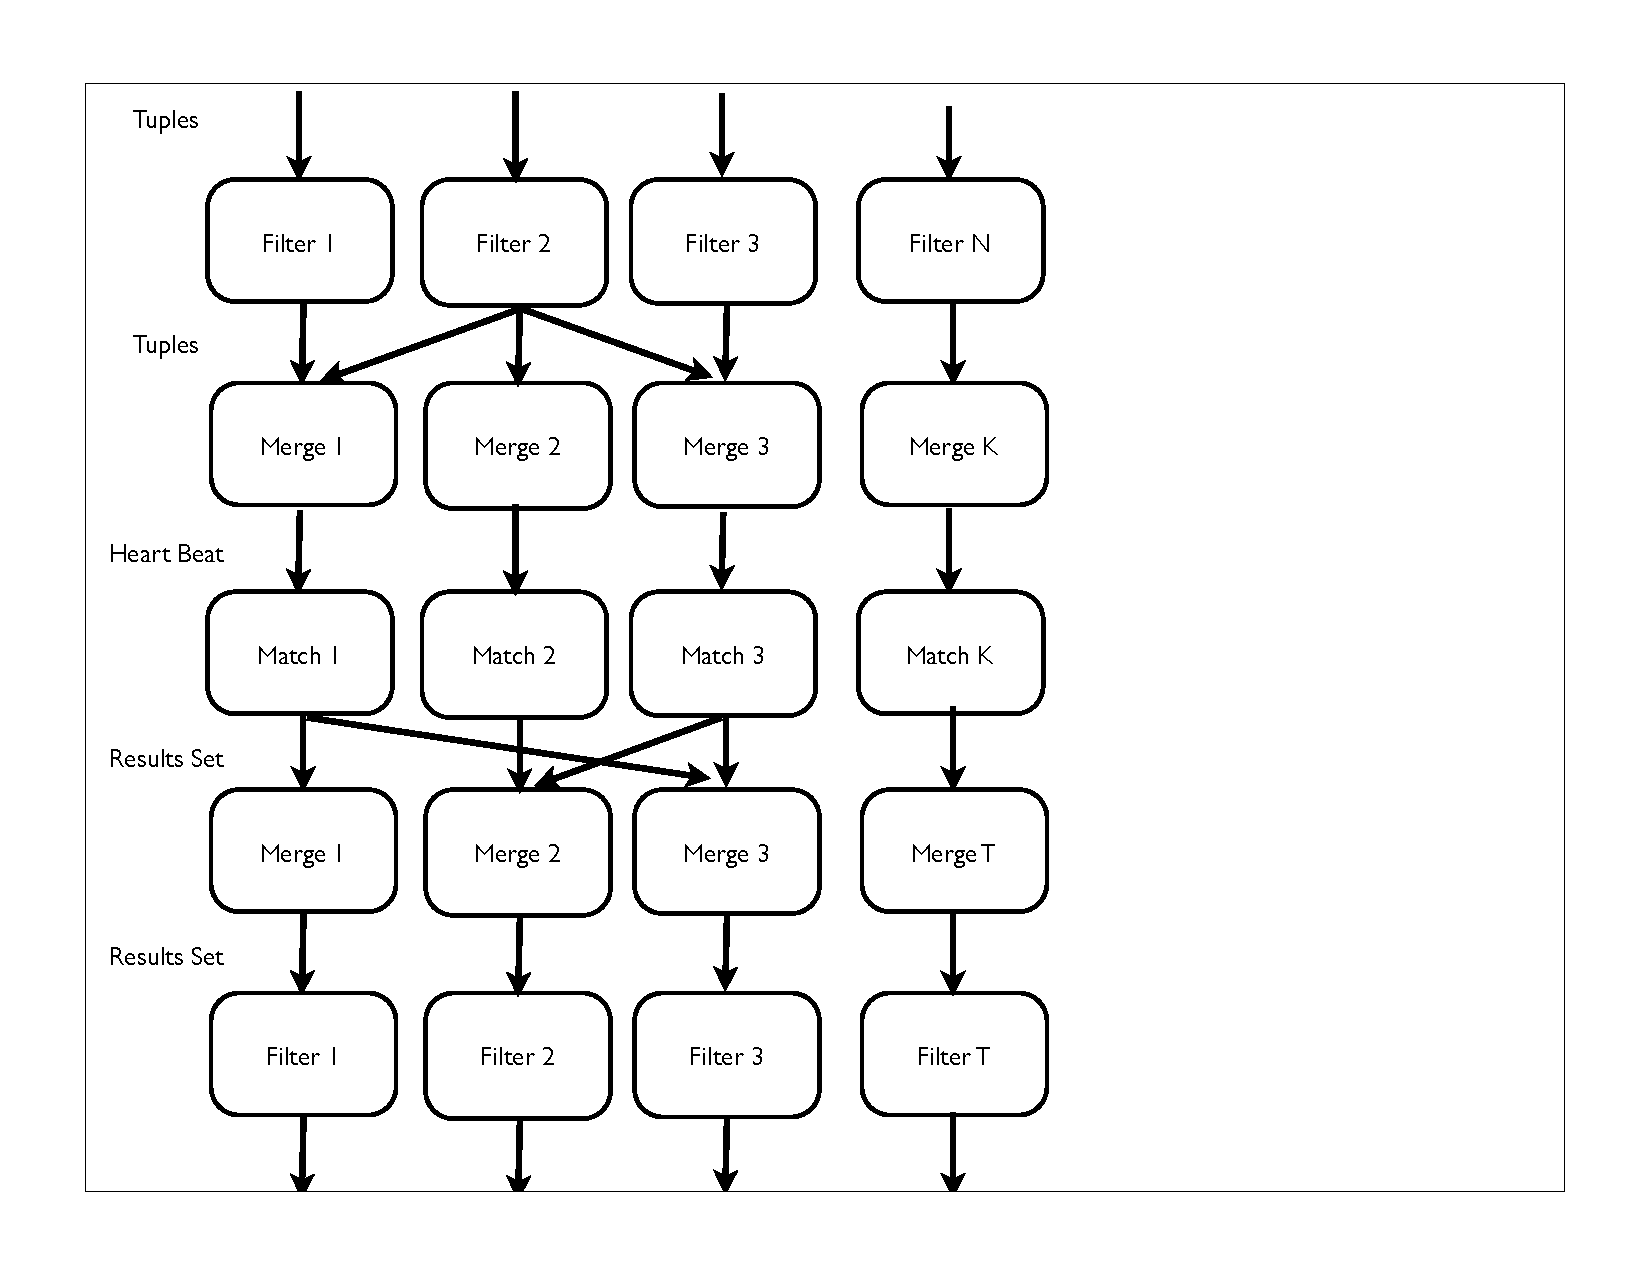
\includegraphics[width=4.50in]{figures/ExchangeFigure.pdf}
%  \caption{Simulator's Execution Path.}
%  \label{fig:overview}
%\end{figure}

%Figure \ref{fig:overview} shows data execution paths and interactions between various components of the Simulator System.

\section{Running Example}

The Stock Exchange Server Simulator uses historical data from previously occurred real stock exchanges and new  buy/sell stock orders from a novel trading strategy. The orders are combined into a single stream of events to emulate the behavior of the trading strategy on the stock exchange. This allows users to evaluate a particular trading strategy. 

The trade requests are combined using historic data replication strategy. Trades, where a historic order matches another historic order or a simulated order matches another simulated order, are executed by matching price and volume of a buy and a sell request. However, when a simulated order can be matched with some historic order, we create a replica of a historic order and match the simulated order with this replicated order.

The Simulator receives two input streams. The first stream consists of trade requests from the historic data file. The second stream consists of the trade requests from the trading algorithms. Each stream is filtered to have only sell, buy and delete orders. The two input streams are mixed to create intermediate stream. The first stream is identical to the historic orders stream after filtering. The second stream is a combination of orders coming from both streams. 

At the next stage, stream tuples are inserted into  \emph{historicView} relations and \emph{combinedView} relations, the relations are matched, and a steam of outputs for each is produced. Each output stream is then cleaned up. If there is a match between a historic order and a simulated order in a combined view relation, a new tuple is inserted into output stream to compensate for the replication of a historic order.


\section{Input Filter}

An input filter is a \emph{stream-to-stream} transformation. It is used to remove undesired updates from input stream or to add updates to the stream based on some input parameters.

The desired functionality for a filter is as follows:

\begin{itemize}
    \item Get an input tuple
    \item Check if a tuple satisfies conditions
    \item If conditions are met, forward tuple to another stream
    \item If conditions are not met, discard the tuple
\end{itemize}

The functionality for an insertion trigger.

\begin{itemize}
    \item Get an input tuple
    \item Check if a tuple satisfies trigger conditions
    \item If conditions are met, create new tuples and forward them to a desired stream
    \item If conditions are not met, ignore the tuple or send it to the stream
\end{itemize}


\noindent The above filters and triggers can be imposed on the same stream and interleaved as desired.

SQL can be used to implement this functionality. For instance, the code to filter out tuples will look like:

\begin{verbatim}   
    INSERT INTO outgoing_stream
    FROM input_stream
    WHERE tuple_condition
\end{verbatim}

\noindent Similarly extra tuples can be added with SQL based on some trigger conditions,

\begin{verbatim}   
    INSERT INTO outgoing_stream: new_tuple_1(tuple), new_tuple_2(tuple), ...
    FROM input_stream
    WHERE trigger_conditio
\end{verbatim}

\noindent where a {\tt new\_tuple\_i(tuple)} statement is a shorthand for a creation of new tuple not necessary based on a tuple from the input stream.

In our example, the Exchange Server has two input streams. One stream is historical data from trades executed at some previous date. The second stream is additional trades coming from the Trading Algorithms. The stream of updates coming from the Trading Algorithms can be controlled by the user (at the moment we assume that users have complete control over the trading algorithms). However, historical data can be dirty and incomplete. We want to give users an ability to restore missing updates or to remove information impurities. For instance, data tuples indicating an order fulfillment can be removed from the system since the Simulator will be able to re-create those tuples by itself. Also if we see a change in some order (the order was partially fulfilled) and we have no reference to such order in the order book, we would want to add such an order to the book.% (the concerns for this operation are noted later).

The two input streams  are a \emph{historic\_input\_stream} stream and a \emph{simulated\_input\_stream} stream. We create filters to remove undesired tuples:

\begin{verbatim}   
    INSERT INTO HFS
    FROM historic_input_stream HS
    WHERE HS.action=='B' &&
          HS.action=='S' &&
          HS.action=='D'
\end{verbatim}

\begin{verbatim}  
    INSERT INTO SFS
    FROM simulated_input_stream SS
    WHERE SS.action=='B' &&
          SS.action=='S' &&
          SS.action=='D'
\end{verbatim}

\noindent We also need to forward these data to the output streams,

\begin{verbatim}   
    INSERT INTO  
    FROM historic_input_stream HS
    WHERE HS.action=='B' &&
          HS.action=='S' &&
          HS.action=='D'
\end{verbatim}

\begin{verbatim}  
    INSERT INTO combined_output
    FROM simulated_input_stream SS
    WHERE SS.action=='B' &&
          SS.action=='S' &&
          SS.action=='D'
\end{verbatim}

\noindent where \emph{historic\_output} and \emph{combined\_output} streams are output streams for the rule matching steps. 


\section{Input Merging}

It is often the case that relevant data is coming from different stream or that streams contains too much data to deal with. We would want to combine (join/union) some input streams or to split a stream based on some parameters of the data to make resultant streams more homogenous. It is also possible to impose future conditions (example windowing) on the input steam. Input Merging is also a \emph{stream-to-stream} transformation.
\\

%Often, once input is received, we would want to combine (join/union) two input streams or to impose future conditions (example windowing) on the input steam. Input Merging is also a \emph{stream-to-stream} transformation.

%, which will allow users to specify those conditions and creates additional relations from them.

The desired functionality of a merging step is simple.
\begin{itemize}
    \item Get tuple from a set of input streams
    \item Forward tuple to output stream
\end{itemize}

\noindent The functionality for the splitting step is as follows.

\begin{itemize}
    \item Get tuple from a set of input streams
    \item Check conditions
    \item Based on the conditions send it to an appropriate stream
\end{itemize}

\noindent In SQL we can combine two input streams if they have the same schema 

\begin{verbatim}   
    input_stream1
    UNION
    input_stream2
    UNION
    ...
    INTO output_stream
\end{verbatim}

\noindent The functionality for the splitting step can also be done in SQL as a set of filters. 

\begin{verbatim}   
    INSERT INTO outgoing_stream_1 
    FROM input_stream
    WHERE condition1
    
    INSERT INTO outgoing_stream_2
    FROM input_stream
    WHERE condition2
    
    ...
\end{verbatim}


A set of streams produced as a result of merging are matched in the Exchange Server. Merging provides a way to combine streams over which matching will be imposed. 

The Exchange Server uses merging to duplicate historical data. This data is merged with the updates coming from new trading strategies.

\begin{verbatim}  
    HFS
    UNION
    SFS
    INTO combinedView
\end{verbatim}

\noindent A \emph{combinedView} stream will contain tuples from the historic data stream and the algorithm's produced stream. A \emph{historicView} stream will contain only tuple from historic data stream. Since we already have this stream we can rename it as follows.

\begin{verbatim}  
    HFS
    INTO historicView
\end{verbatim}


In many cases we will want to distinguish between tuples coming from different streams. This requires expanding the schema of the update tuples. 

\begin{verbatim}  
    (SELECT augmented_tuple_historic
     FROM HFS hs)
    UNION
    (SELECT augmented_tuple_simulated
     FROM SFS ss)
    INTO combinedView
\end{verbatim}

Here constructs \emph{augmented\_tuple\_historic} and \emph{augmented\_tuple\_simulated} are a short for:

\begin{verbatim}
    augmented_tuple_historic -> hs.id, hs.time, hs.action,
                            hs.volume, hs.price, source="hist"
    augmented_tuple_simulated -> ss.id, ss.time, ss.action,
                            ss.volume, ss.price, source="sim"
\end{verbatim}

The above merging allows us to expand a tuples' schema, to include the tuples source. 

The above merging step produces two streams: \emph{combinedView} and\emph{historicView}. A \emph{historicView} stream contains filtered tuple only from a \emph{HFS} stream. A \emph{combinedView} stream contains tuples from both a \emph{HFS} and a \emph{SFS} streams. The \emph{combinedView} stream's schema is expanded to include the source stream.


\section{Simulator Rules}

Simulator rules are a set of user definitions on how to create relations from input streams. They also show how to reduce the relations and to produce a stream of output events.

\subsection{Stream to Relations}
All actions performed so far were \emph{stream-to-stream} actions. These actions allowed us to manipulate streams of incoming data to create a stream of updates for a set of relations. Next step is to materialize this stream into a set of relations and to apply user defined rules to them. 

In our running example we would want to visualize the bid and the ask order books into two relations. Each stream produced at an Input Merging stage will have a bid and an ask books.

The bid order book is visualized as a set of buy requests over unbounded time frame.

\begin{verbatim}  
    SELECT * as bids_historicView
    FROM historicView hv
    RANGE UNBOUNDED
    WHERE hv.action=='B'
\end{verbatim}

\noindent Similarly for an ask relation.

\begin{verbatim}  
    SELECT * as asks_historicView
    FROM historicView hv
    RANGE UNBOUNDED
    WHERE hv.action=='S'
\end{verbatim}

\noindent The bid and the ask relations for the \emph{compbineView} stream are done similarly.

\begin{verbatim}  
    SELECT * as bids_combinedView
    FROM combinedView cv
    RANGE UNBOUNDED
    WHERE cv.action=='B'
\end{verbatim}

\noindent And the ask relation

\begin{verbatim}  
    SELECT * as asks_combinedView
    FROM combinedView cv
    RANGE UNBOUNDED
    WHERE cv.action=='S'
\end{verbatim}

\noindent The ask and bid relations are updated with new tuples from the stream. The stream also contains user requests to remove some tuples from those relations. This is can be accomplished with the following deletes.

\begin{verbatim}  
    DELETE *
    FROM asks_historicView av
    WHERE av.id = hv.id
            (SELECT * 
             FROM historicView
             RANGE NOW
             WHERE historicView.action='D') as hv  

    DELETE *
    FROM bids_historicView bv
    WHERE bv.id = hv.id
            (SELECT * 
             FROM historicView
             RANGE NOW
             WHERE historicView.action='D') as hv 
\end{verbatim}

Similarly we can update order-book relations for the \emph{combinedView} stream.

\begin{verbatim}  
    DELETE *
    FROM asks_combinedView av
    WHERE av.id = cv.id
            (SELECT * 
             FROM combinedView
             RANGE NOW
             WHERE combinedView.action='D') as cv  

    DELETE *
    FROM bids_combinedView bv
    WHERE bv.id = cv.id
            (SELECT * 
             FROM combinedView
             RANGE NOW
             WHERE combinedView.action='D') as cv 
\end{verbatim}


\subsection{Rule Application}

The main component of our system is its ability to apply a set of user defined rules to a set of relations resulting in a stream of output tuples. This provides users with an ability to manipulate the relations. The rules define how the output stream for a group of relations is produced and how the existent relations are changed. 

\begin{verbatim}
    REDUCE_LOOP [WHILE condition | TIMES number]
    FROM [NEW] relation1, [NEW] relation2, ... 
    WHEN condition1
        (set of statements to be executed)
    WHEN condition2
        ...
    WITH HEARTBEAT ON (tuple identifier)
    EVERY [number TUPLE | time INTERVAL] IN relation 
\end{verbatim}

The {\tt REDUCE\_LOOP} statement shows with a simple set of statements give the consequences of some events being true. This statement gives an ability for a set of actions to be executed, when the conditions are satisfied. The conditions are specified by the {\tt WHEN} clause followed by a set of SQL statements to be executed in case the condition is true. The {\tt REDUCE\_LOOP} statement can be executed repeatedly when conditions {\tt WHILE} or {\tt TIMES} are present. A {\tt WHILE} predicate followed by a condition indicates that the statements should be executed while the conditions are true. A {\tt TIMES} predicate indicates how many times the conditions should be executed. A {\tt FROM} predicate indicates what tables the data is coming from, on which the {\tt WHILE} condition is applied. A field specifier {\tt NEW} indicates that the content of the table should be updated on every iteration. The need to update can come as a result of new tuples inserted into a relation caused by the execution of the statements.   

In our running example of the Exchange Server, we provide rules where if the price on the best ask order and best bid order match we remove/update them from/in the tables and send consequences of the update to the output stream.

Before we start matching we need to define relations we will be using later.

\begin{verbatim}      
    SELECT * as min_bid_price
    FROM bids_historicView bhv
    WHERE bhv.price = (SELECT min(price) FROM  bids_historicView))
    
    SELECT * as top_bid
    FROM min_bid_price mbp
    WHERE mbp.time = (SELECT min(time) FROM min_bid_price)
    
    SELECT * as max_ask_price
    FROM asks_historicView ahv
    WHERE ahv.price = (SELECT max(price) FROM  asks_historicView))
    
    SELECT * as top_ask
    FROM max_ask_price map
    WHERE map.time = (SELECT min(time) FROM max_ask_price)
\end{verbatim}

We can start matching using above specification.

\begin{verbatim}  
    REDUCE_LOOP WHILE top_bid.price<=top_ask.price
    FROM NEW top_bid, NEW top_ask
    WHEN top_bid.volume = top_ask.volume 
            (DELETE * FROM bids_historicView bhv 
                      WHERE bhv.id = top_bid.id,
             DELETE * FROM asks_historicView ahv 
                      WHERE ahv.id = top_ask.id,
             INSERT INTO historic_output: 
                        create_F(top_bid), create_F(top_ask))
    WHEN top_bid.volume < top_ask.volume 
            (DELETE * FROM bids_historicView bhv 
                      WHERE bhv.id = top_bid.id,
             INSERT INTO asks_historicView: create_E_update(top_ask) 
                ON DUPLICATE KEY UPDATE id = top_ask.id
             INSERT INTO historic_output:
                        create_F(top_bid), create_E(top_bid))
    WHEN top_bid.volume > top_ask.volume 
            (DELETE * FROM asks_historicView ahv 
                      WHERE ahv.id = top_ask.id,
             INSERT INTO bids_historicView: create_E_update(top_bid) 
                 ON DUPLICATE KEY UPDATE id = top_bid.id
             INSERT INTO historic_output:
                        create_F(top_ask), create_E(top_bid))
    WITH HEARTBEAT ON *
    EVERY 1 TUPLE IN historicView
\end{verbatim}

In the above we compute {\tt top\_bid} and {\tt top\_ask} tables containing the best ask tuple and the best bid tuple on every iteration. The \emph{create\_F(top\_bid)}, \emph{create\_F(top\_ask)}, \emph{create\_E(top\_bid)}, \emph{create\_E(top\_ask)}, \emph{create\_E\_update(top\_ask)}, and \emph{create\_E\_update(top\_bid)} statements are a short hand for:

\begin{verbatim}
    create_F(top_bid) -> top_bid.id, top_bid.time, top_bid.action='F',
                            top_bid.volume, top_bid.price
    create_F(top_ask) -> top_ask.id, top_ask.time, top_ask.action='F',
                            top_ask.volume, top_ask.price
    create_E(top_bid) -> top_bid.id, top_bid.time, top_bid.action='E',
                            top_ask.volume, top_bid.price
    create_E(top_ask) -> top_ask.id, top_ask.time, top_ask.action='E',
                            top_bid.volume, top_ask.price
    create_E_update(top_bid) -> top_bid.id, top_bid.time,
                    top_bid.action='E', top_bid.volume - top_ask.volume,
                    top_bid.price
    create_E_update(top_ask) -> top_ask.id, top_ask.time,
                    top_ask.action='E', top_ask.volume - top_bid.volume,
                    top_ask.price
\end{verbatim}


The {\tt REDUCE\_LOOP} statements proceeds to iterate through the loop until the top bid and the top ask tuples cannot be matched on price. Depending on the quantity of stocks in the bid and the ask order the consequences of matching differ. The {\tt REDUCE\_LOOP} matching rule is initiated on every update tuple to the \emph{historicView} stream. 

Now we can specify the matching rule for the \emph{combinedView} stream.

\begin{verbatim}      
    SELECT * as min_bid_price
    FROM bids_combinedView bhv
    WHERE bhv.price = (SELECT min(price) FROM  bids_historicView))
    
    SELECT * as top_bid
    FROM min_bid_price mbp
    WHERE mbp.time = (SELECT min(time) FROM min_bid_price)
    
    SELECT * as max_ask_price
    FROM asks_combinedView ahv
    WHERE ahv.price = (SELECT max(price) FROM  asks_historicView))
    
    SELECT * as top_ask
    FROM max_ask_price map
    WHERE map.time = (SELECT min(time) FROM max_ask_price)
\end{verbatim}

The {\tt REDUCE\_LOOP} statement for the \emph{combinedView} stream is similar to the one above. 

\begin{verbatim}  
    REDUCE_LOOP WHILE top_bid.price<=top_ask.price
    FROM NEW top_bid, NEW top_ask
    WHEN top_bid.volume = top_ask.volume 
            (DELETE * FROM bids_combinedView bcv 
                      WHERE bcv.id = top_bid.id,
             DELETE * FROM asks_combinedView acv 
                      WHERE acv.id = top_ask.id,
             INSERT INTO combined_output:
                      SELECT create_B(top_bid), create_F(top_bid)
                      FROM top_bid t
                      WHERE t.source="hist" && top_ask.source="sim"
             INSERT INTO combined_output:
                      SELECT create_S(top_ask), create_F(top_ask)
                      FROM top_ask t
                      WHERE t.source="hist" && top_bid.source="sim"
             INSERT INTO combined_output: 
                      SELECT create_F(top_bid)
                      FROM top_bids
                      WHERE top_bids.source="sim"
             INSERT INTO combined_output: 
                      SELECT create_F(top_ask)
                      FROM top_ask
                      WHERE top_ask.source="sim")
    WHEN top_bid.volume < top_ask.volume 
            (DELETE * FROM bids_combinedView bcv 
                      WHERE bcv.id = top_bid.id,
             INSERT INTO asks_combinedView: create_E_update(top_ask)
                ON DUPLICATE KEY UPDATE id = top_ask.id
             INSERT INTO combined_output:
                      SELECT create_B(top_bid), create_F(top_bid)
                      FROM top_bid t
                      WHERE t.source="hist" && top_ask.source="sim"
             INSERT INTO combined_output:
                      SELECT create_S(top_ask), create_F(top_ask)
                      FROM top_ask t
                      WHERE t.source="hist" && top_bid.source="sim"
             INSERT INTO combined_output: 
                      SELECT create_F(top_bid)
                      FROM top_bids
                      WHERE top_bids.source="sim"
             INSERT INTO combined_output: 
                      SELECT create_F(top_ask)
                      FROM top_ask
                      WHERE top_ask.source="sim")
    WHEN top_bid.volume > top_ask.volume 
            (DELETE * FROM asks_combinedView acv 
                      WHERE acv.id = top_ask.id,
             INSERT INTO bids_combinedView: create_E(top_bid) 
                 ON DUPLICATE KEY UPDATE id = top_bid.id
             INSERT INTO combined_output:
                     SELECT create_B(top_bid), create_F(top_bid)
                     FROM top_bid t
                     WHERE t.source="hist" && top_ask.source="sim"
             INSERT INTO combined_output:
                     SELECT create_S(top_ask), create_F(top_ask)
                     FROM top_ask t
                     WHERE t.source="hist" && top_bid.source="sim"
             INSERT INTO combined_output: 
                     SELECT create_F(top_bid)
                     FROM top_bids
                     WHERE top_bids.source="sim"
             INSERT INTO combined_output: 
                     SELECT create_F(top_ask)
                     FROM top_ask
                     WHERE top_ask.source="sim")
    WITH HEARTBEAT ON *
    EVERY 1 TUPLE IN combinedView
\end{verbatim}

Similarly the \emph{create\_F(top\_bid)}, \emph{create\_F(top\_ask)}, \emph{create\_E(top\_bid)}, \emph{create\_E(top\_ask)}, \emph{create\_E\_update(top\_ask)}, and \emph{create\_E\_update(top\_bid)} statements stand for:

\begin{verbatim}
    create_F(top_bid) -> top_bid.id, top_bid.time, top_bid.action='F',
                            top_bid.volume, top_bid.price
    create_F(top_ask) -> top_ask.id, top_ask.time, top_ask.action='F',
                            top_ask.volume, top_ask.price
    create_E(top_bid) -> top_bid.id, top_bid.time, top_bid.action='E',
                            top_ask.volume, top_bid.price
    create_E(top_ask) -> top_ask.id, top_ask.time, top_ask.action='E',
                            top_bid.volume, top_ask.price
    create_E_update(top_bid) -> top_bid.id, top_bid.time,
                    top_bid.action='E', top_bid.volume - top_ask.volume,
                    top_bid.price
    create_E_update(top_ask) -> top_ask.id, top_ask.time,
                    top_ask.action='E', top_ask.volume - top_bid.volume,
                    top_ask.price
\end{verbatim}

\noindent The \emph{create\_B(top\_bid)} and the \emph{create\_S(top\_ask)} statements standing for 

\begin{verbatim}
    create_B(top_bid) -> top_bid.id+1, top_bid.time, top_bid.action='B',
                            top_ask.volume, top_bid.price
    create_S(top_ask) -> top_ask.id+1, top_ask.time, top_ask.action='S',
                            top_bid.volume, top_ask.price
\end{verbatim}

The matching rule for the \emph{combinedView} stream is more complicated than the matching rule for the \emph{historicView} stream. This is caused by the need to insert a duplicate of a matched historic tuple into the output stream.

\subsection{REDUCE\_LOOP Simplifications}

It is possible to simplify the functionality of the {\tt REDUCE\_LOOP} statement by removing a {\tt HEARTBEAT} condition from it. The purpose of the {\tt HEARTBEAT} is to indicate when the {\tt REDUCE\_LOOP} statement should be executed. 

The {\tt HEARTBEAT} condition is tied to a stream. This means we can remove it from the definition of the {\tt REDUCE\_LOOP} statement and create a stand alone statement to be imposed on any stream. 

\begin{verbatim}
    APPLY HEARTBEAT TO reduce_loop_name1, reduce_loop_name2, ...
    ON stream
    EVERY [number TUPLE | time INTERVAL] IN relation
\end{verbatim}

\noindent Here a \emph{reduce\_loop\_name1} name indicates the name of a reduce loop statement. This condition imposed on a stream will trigger {\tt REDUCE\_LOOP} statements by the given names. 

Consequently a {\tt REDUCE\_LOOP} statement will be modified as follows.

\begin{verbatim}
    REDUCE_LOOP name [WHILE condition | TIMES number]
    FROM [NEW] relation1, [NEW] relation2, ... 
    WHEN condition1
        (set of statements to be executed)
    WHEN condition2
        ...
\end{verbatim}

\section{Output Merging}

The Output Merging step is similar to the Input Merging step. The idea is to take streams produced at the reduce loop step and combine them into desirable output streams. This is done similarly to Input Merging with either joining of two streams on a set of attributes or doing a union of two streams.

\begin{verbatim}   
    input_stream1
    UNION
    input_stream2
    UNION
    ...
    INTO output_stream
\end{verbatim}

The Exchange Server outputs only one stream of updates. Thus, when matching occurs over a set of relations, they are combined into a single stream.

\begin{verbatim}
    historic_output
    UNION
    (SELECT filtered_tuple
    FROM combined_output co)
    INTO output_stream
\end{verbatim}

\noindent A \emph{historic\_output} stream is a stream resulting from the matching rule imposed on the \emph{historicView} stream. A \emph{combined\_output} stream is a stream produce by the matching rule imposed on the \emph{combinedView} stream. We cannot combine the two streams, because they have different schemas. A \emph{combined\_output} stream has an extra field called \emph{source}, which needs to be removed first. A \emph{filtered\_tuple} parameter indicates a tuple from the \emph{combined\_output} stream with a \emph{source} field removed.


\section{Output Filtering} 

An Output filter is a step for the last minute changes to the outgoing data. In some ways it is very similar to the input filter. It can add or project away fields in the stream. Additionally it can impose user defined functions to the tuples in the stream.

\begin{verbatim}
    APPLY user_function(*)
    FROM input_stream
    TO   output_stream 
\end{verbatim}

This functionality allows for users to take a tuple from the stream and change some of its parameters.

We know that during stock trading the stock prices respond to high volume trades by the increase in their sale price. The users can create a filter to emulate this. For example, when there is a high volume stock movement in the \emph{combined\_output} stream users might want to increase price field value in all stock transactions by a small amount for a given time frame. Thus we can add the following filter

\begin{verbatim}
    APPLY price_change(*)
    FROM output_stream
    TO   final_output 
\end{verbatim}

Here a \emph{price\_change(*)} function is defined on the output tuple. The output of the function is a changed tuple. In this case the \emph{price} field is dynamically changed to reflect the potential stock price increase/decrease.

The function in the {\tt APPLY} statement can be dynamic. The function can monitor some streams and based on the trigers the it will change its internal parameters to increase or decrease the stock price. In this case we might have a trigger, 

\begin{verbatim}
    SELECT *
    FROM combined_output co
    WHERE co.action="B" && co.volume>1000
\end{verbatim}

\noindent that indicated when to increase the price. 

\section{Execution Order}

Every tuple processed by the simulator in a given order. This order is defined by the users in the form of stream/table dependencies. The dependencies are a pairwise constraints indicating that a tuple should be processed at a given stage(s) before being moved at a different stream. The dependences form a path from the input stream to the output stream. The set of such paths forms a directed acyclic graph. There is nothing in the definition of the constraints that restricts a graph to be acyclic. The existence of the reduce loop step provided the system with the necessary iteration capabilities. 

Any two stages can be executed in parallel unless they lie on the same path. If two paths converge at some stage, the users have to specify if the streams should to be synchronized, parallelized or ordered at that point.

The pairwise constraints can be inferred from the SQL statement analyses. A {\tt FROM} clause in a {\tt SELECT} or an {\tt INSERT} statements indicates a stream or a relation that depends on a stream indicated by {\tt INTO} clause. A {\tt UNION} clause indicates a point in a DAG where several paths converge.

The {\tt UNION} clause can be re-written in the following format.

\begin{verbatim}
    UNION [PARALLEL | ORDERED | SYNCHRONIZED]
            stream_name1, stream_name2, ...
    INTO result_stream
\end{verbatim}   

\noindent Here the {\tt PARALLEL} keyword indicates no order imposed on the tuples coming from different streams. This indicates that two path are independent of each other and can still be executed in parallel. The {\tt ORDERED} keyword indicates that incoming tuples should be processed in the order of the stream arrangement in the {\tt UNION} clause. The {\tt SYNCHRONIZED} keyword indicates that if there is a common ancestor for the two paths all the tuples generated by this source should wait until all the path either converge at this point or stop execution, before releasing the buffered tuples to the next stream. 

The {\tt REDUCE\_LOOP} statement is a loop that influences a set of streams and relations during its execution. These streams and relations are made unavailable (locked) to the external changes. 

A tuple moves through the simulator using a push-through policy. When a tuple is received, it moves from stream to stream until it is either moved to an output stream or no new tuple is created.

\section{Alternative Simulator Structures}

The above simulator system creates a fair amount of data replication. This leads to a repetition of work. For example, in our example of the Exchange Simulator we have two similar reduce loops. The reduce loop responsible for handling data coming from the \emph{combinedView} stream repeats a lot of matches between historic tuples. Those matches are ignored by the reduce loop, since they are duplicated in the first reduce loop based on the \emph{historicView} stream. 

Here we will present alternative approaches to the system design that reduces the amount of repeated work. 

\subsection{Rule Reliance}
The first strategy will rely on creating elaborate rule structure that will enables uses to accomplish the same goals without any data replication. The down side of this approach is that it creates elaborate schemas for the internal streams. Additionally, the matching rules will have to be more complicated.  

\subsubsection{Input Filtering}

The input filtering component remains the same. The purpose of the filter is to remove tuples users do not care about. This need does not change with this approach. 

\subsubsection{Input Merging}

The previous approach used this step to replicate the data into the various streams. This approach will merge the streams to limit the amount of replication. The semantics of the step will remain the same but the implications will differ. In this step all the streams will be merged if they need to be used together in the later reduce step.


In the exchange simulator we will have. 
\begin{verbatim}
    (SELECT augmented_tuple_historic
     FROM HFS hs)
    UNION
    (SELECT augmented_tuple_simulated
     FROM SFS ss)
    INTO combinedView 
\end{verbatim}

The side effect of not replicating data is the change and unification of schemas for each input stream. 

Here \emph{augmented\_tuple\_historic} and \emph{augmented\_tuple\_simulated} constructs are a short hand for:

\begin{verbatim}
    augmented_tuple_historic -> hs.id, hs.time, hs.action,
                            hs.volume, hs.price, source="hist",
                            base_volume=hs.volume, current_volume=0
    augmented_tuple_simulated -> ss.id, ss.time, ss.action,
                            ss.volume, ss.price, source="sim"hist",
                            base_volume=hs.volume, current_volume=0
\end{verbatim}

As we can see the schema is more complex compared to similar augmented tuples in the previous example.

\subsubsection{Simulator Rules}

The simulator rules are similar to the approach above. First we need to visualize and separate data into the tables needed in the later reduce step. This step in the Exchange Simulator is identical to the step of separating data into tables for the \emph{combinedView} stream and is omitted here.

The specification for the {\tt REDUCE\_LOOP} statement will not change, however achieving the same functionality will be more difficult. 

\begin{verbatim}
    REDUCE_LOOP name [WHILE condition | TIMES number]
    FROM [NEW] relation1, [NEW] relation2, ... 
    [WHEN condition1
        (set of statements to be executed)]
\end{verbatim}

The Exchange Simulator design of the {\tt REDUCE\_LOOP} statement will change to account for more complicated matching. But before we begin we need to show how helper relations are calculated.

\begin{verbatim}      
    SELECT * as min_bid_price
    FROM bids_combinedView bhv
    WHERE bhv.price = (SELECT min(price) 
                       FROM  bids_combinedView bv"))
    
    SELECT * as top_bid
    FROM min_bid_price mbp
    WHERE mbp.time = (SELECT min(time) FROM min_bid_hist_price)
    
    SELECT * as min_bid_sim_price
    FROM bids_combinedView bhv
    WHERE bhv.price = (SELECT min(price) 
                       FROM  bids_combinedView bv
                       WHERE bv.current_volume<bv.base_volume))
    
    SELECT * as top_sim_bid
    FROM min_bid_sim_price mbp
    WHERE mbp.time = (SELECT min(time) FROM min_bid_sim_price)
    
    SELECT * as max_ask_price
    FROM asks_combinedView ahv
    WHERE ahv.price = (SELECT max(price) 
                       FROM  asks_combinedView av)
    
    SELECT * as top_ask
    FROM max_ask_price map
    WHERE map.time = (SELECT min(time) FROM max_ask_price)
    
    SELECT * as max_ask_sim_price
    FROM asks_combinedView asv
    WHERE asv.price = (SELECT max(price) 
                       FROM  asks_combinedView av
                       WHERE bv.current_volume<bv.base_volume))
    
    SELECT * as top_sim_ask
    FROM max_ask_sim_price map
    WHERE map.time = (SELECT min(time) FROM max_ask_sim_price)
\end{verbatim}

Now we can turn back to the {\tt REDUCE\_LOOP} statement.

\begin{verbatim}  
    REDUCE_LOOP WHILE (top_bid.price<=top_ask.price && 
                        top_bid="hist" && top_ask="hist") ||
                      (top_bid.price<=top_ask.price && 
                        top_bid="sim" && top_ask="sim") ||
                      (top_bid.price<=top_sim_ask.price && 
                        top_bid="sim" && top_ask="hist") ||
                      (top_sim_bid.price<=top_ask.price && 
                        top_bid="hist" && top_ask="sim")
    FROM NEW top_bid, NEW top_ask, NEW top_sim_bid, NEW top_sim_ask
    WHEN (top_bid="hist" && top_ask="hist" ||
                                top_bid="sim" && top_ask="sim") &&
           top_bid.volume = top_ask.volume
           (DELETE * FROM bids_combinedView bcv 
                     WHERE bcv.id = top_bid.id,
            DELETE * FROM asks_combinedView acv 
                     WHERE acv.id = top_ask.id,
            INSERT INTO combined_output:
                     create_F(top_bid), create_F(top_ask))
    WHEN (top_bid="hist" && top_ask="hist" ||
               top_bid="sim" && top_ask="sim") &&
           top_bid.volume < top_ask.volume                     
           (DELETE * FROM bids_combinedView bcv 
                     WHERE bcv.id = top_bid.id,
            INSERT INTO asks_combinedView: update_S(top_ask) 
                     ON DUPLICATE KEY UPDATE id = top_ask.id
            INSERT INTO combined_output: 
                     create_F(top_bid), create_E(top_ask))
     WHEN (top_bid="hist" && top_ask="hist" ||
               top_bid="sim" && top_ask="sim") &&
            top_bid.volume > top_ask.volume                     
           (DELETE * FROM asks_combinedView acv 
                     WHERE acv.id = top_ask.id,
            INSERT INTO asks_combinedView: update_B(top_bid) 
                     ON DUPLICATE KEY UPDATE id = top_bid.id
            INSERT INTO combined_output: 
                     create_E(top_bid), create_F(top_ask))
     WHEN (top_bid="sim" && top_ask="hist" &&
              top_bid.volume = 
                (top_sim_ask.base_volume - top_sim_ask.current_volume))
            (DELETE * FROM bids_combinedView bcv
                      WHERE bcv.id = top_bids.id
             DELETE * FROM asks_combinedView acv
                      WHERE acv.id = 
                        (SELECT *
                         FROM top_sim_ask t
                         WHERE t.source="sim")
             INSERT INTO asks_combinedView: 
                      (SELECT update_S(top_sim_ask)
                       FROM top_sim_ask t
                       WHERE t.source="hist") tuple
                      ON DUPLICATE KEY UPDATE id= tuple.id
             INSERT INTO combined_output:
                     (SELECT create_S(top_sim_ask), create_F(top_sim_ask)
                        FROM top_sim_ask t
                        WHERE t.source="hist")
             INSERT INTO combined_output:
                     (SELECT create_s_F(top_sim_ask)
                      FROM top_sim_ask t
                      WHERE t.source="sim")
             INSERT INTO combined_output:
                     create_F(top_bid))
     WHEN (top_bid="sim" && top_ask="hist" &&
               top_bid.volume < 
               (top_sim_ask.base_volume - top_sim_ask.current_volume)) 
            (DELETE * FROM bids_combinedView bcv
                      WHERE bcv.id = top_bids.id 
              INSERT INTO asks_combinedView: 
                        (SELECT update_S(top_sim_ask)
                         FROM top_sim_ask t
                         WHERE t.source="hist") tuple
                        ON DUPLICATE KEY UPDATE id= tuple.id
               INSERT INTO asks_combinedView:
                        (SELECT create_s_S(top_sim_ask)
                         FROM top_sim_ask t
                         WHERE t.source="sim") tuple
                        ON DUPLICATE KEY UPDATE id = tuple.id
               INSERT INTO combined_output:
                       (SELECT create_S(top_sim_ask), create_F(top_sim_ask)
                         FROM top_sim_ask t
                         WHERE t.source="hist")
               INSERT INTO combined_output:
                       (SELECT create_E(top_sim_ask)
                        FROM top_sim_ask t
                        WHERE t.source="sim")
               INSERT INTO combined_output:
                        create_F(top_bid))
    WHEN (top_bid="sim" && top_ask="hist" &&
               top_bid.volume > 
                (top_sim_ask.base_volume - top_sim_ask.current_volume))
         (INSERT INTO bids_combinedView: create_B(top_bid)
                 ON DUPLICATE KEY UPDATE id= top_bid.id
          INSERT INTO asks_combinedView: 
                  (SELECT update_S(top_sim_ask)
                   FROM top_sim_ask t
                   WHERE t.source="hist") tuple
                 ON DUPLICATE KEY UPDATE id= tuple.id
          DELETE * FROM asks_combinedView acv
                   WHERE acv.id = 
                      (SELECT *
                       FROM top_sim_ask t
                       WHERE t.source="sim")
          INSERT INTO combined_output:
                  (SELECT create_u_S(top_sim_ask), create_u_F(top_sim_ask)
                   FROM top_sim_ask t
                   WHERE t.source="hist")
          INSERT INTO combined_output:
                  (SELECT create_s_F(top_sim_ask)
                   FROM top_sim_ask t
                   WHERE t.source="sim")
          INSERT INTO combined_output:
                   create_s_E(top_bid))
    WHEN (top_bid="hist" && top_ask="sim" &&
            top_sim_bids.current_volume = top_ask.volume)
         (DELETE * FROM asks_combinedView acv
                   WHERE acv.id = top_asks.id
          DELETE * FROM bids_combinedView bcv
                   WHERE bcv.id = 
                      (SELECT *
                       FROM top_sim_bid t
                       WHERE t.source="sim")
          INSERT INTO bids_combinedView: 
                  (SELECT update_B(top_sim_bid)
                   FROM top_sim_bid t
                   WHERE t.source="hist") tuple
                 ON DUPLICATE KEY UPDATE id= tuple.id
             INSERT INTO combined_output:
                     (SELECT create_B(top_sim_bid), create_F(top_sim_bid)
                        FROM top_sim_bid t
                        WHERE t.source="hist")
             INSERT INTO combined_output:
                     (SELECT create_b_F(top_sim_bid)
                        FROM top_sim_bid t
                        WHERE t.source="sim")
             INSERT INTO combined_output:
                     create_F(top_ask))
     WHEN (top_bid="hist" && top_ask="sim" &&
             (top_sim_ask.base - top_sim_bids.current_volume)
              < top_ask.volume)
        (INSERT INTO asks_combinedView create_S(top_ask)
            ON DUPLICATE KEY UPDATE id=top_ask.id
         DELETE * FROM bids_combinedView bcv
                  WHERE bcv.id = 
                     (SELECT *
                      FROM top_sim_bid t
                      WHERE t.source="sim")
         INSERT INTO bids_combinedView: 
                     (SELECT update_B(top_sim_bid)
                      FROM top_sim_bid t
                      WHERE t.source="hist") tuple
                ON DUPLICATE KEY UPDATE id= tuple.id
         INSERT INTO combined_output:
                     (SELECT create_u_B(top_sim_bid), create_u_F(top_sim_bid)
                      FROM top_sim_bid t
                      WHERE t.source="hist")
         INSERT INTO combined_output:
                     (SELECT create_b_F(top_sim_bid)
                      FROM top_sim_bid t
                      WHERE t.source="sim")           
         INSERT INTO combined_output:
                      create_E(top_ask))
     WHEN (top_bid="hist" && top_ask="sim" &&
              (top_sim_ask.base - top_sim_bids.current_volume)
               > top_ask.volume)              
        (DELETE * FROM asks_combinedView acv
                  WHERE acv.id = top_asks.id
         INSERT INTO bids_combinedView: 
                     (SELECT update_B(top_sim_bid)
                      FROM top_sim_bid t
                      WHERE t.source="hist") tuple
                ON DUPLICATE KEY UPDATE id= tuple.id
         INSERT INTO bids_combinedView: 
                     (SELECT create_b_B(top_sim_bid)
                      FROM top_sim_bid t
                      WHERE t.source="sim") tuple
                  ON DUPLICATE KEY UPDATE id= tuple.id
         INSERT INTO combined_output:
                     (SELECT create_B(top_sim_bid), create_F(top_sim_bid)
                      FROM top_sim_bid t
                      WHERE t.source="hist")
         INSERT INTO combined_output:
                     (SELECT create_E(top_sim_bid)
                      FROM top_sim_bid t
                      WHERE t.source="sim")
         INSERT INTO combined_output:
                      create_F(top_ask))      
\end{verbatim}

The \emph{create\_X()} and {updates} statements are a short hand for the following tuples:

\begin{verbatim}
create_F(top_bid) -> top_bid.id, top_bid.time, top_bid.action="F",
                     top_bid.volume, top_bid.price,
                     top_bid.base_volume, top_bid.current_volume
                     
create_F(top_ask) -> top_ask.id, top_ask.time, top_ask.action="F",
                     top_ask.volume, top_ask.price,
                     top_ask.base_volume, top_ask.current_volume
                     
update_S(top_ask) -> top_ask.id, top_ask.time, top_ask.action,
                     top_ask.volume - top_bid.volume, top_ask.price,
                     top_ask.base_volume, top_ask.current_volume
                     
create_E(top_ask) -> top_ask.id, top_ask.time, top_ask.action="E",
                     top_bid.volume, top_ask.price,
                     top_ask.base_volume, top_ask.current_volume
                     
update_B(top_bid) -> top_bid.id, top_bid.time, top_bid.action,
                     top_bid.volume - top_ask.volume, top_bid.price,
                     top_bid.base_volume, top_bid.current_volume
                     
create_E(top_bid) -> top_bid.id, top_bid.time, top_bid.action="E",
                     top_ask.volume, top_bid.price,
                     top_bid.base_volume, top_bid.current_volume
                     
update_S(top_sim_ask) -> top_sim_ask.id, top_sim_ask.time,
                         top_sim_ask.action, top_sim_ask.volume, 
                         top_sim_ask.price, top_sim_ask.base_volume, 
                         top_sim_ask.current_volume + top_bid.volume
                         
create_S(top_sim_ask) -> top_sim_ask.id+1, top_sim_ask.time,
                         top_sim_ask.action, top_bid.volume, 
                         top_sim_ask.price, top_sim_ask.base_volume, 
                         top_sim_ask.current_volume
                         
create_F(top_sim_ask) -> top_sim_ask.id+1, top_sim_ask.time,
                         top_sim_ask.action="F", top_bid.volume, 
                         top_sim_ask.price, top_sim_ask.base_volume, 
                         top_sim_ask.current_volume

create_u_S(top_sim_ask) -> top_sim_ask.id+1, top_sim_ask.time,
                         top_sim_ask.action, 
                         top_sim_ask.base_volume - top_sim_ask.current_volume, 
                         top_sim_ask.price, top_sim_ask.base_volume, 
                         top_sim_ask.current_volume

create_u_F(top_sim_ask) -> top_sim_ask.id+1, top_sim_ask.time,
                         top_sim_ask.action="F", 
                         top_sim_ask.base_volume - top_sim_ask.current_volume, 
                         top_sim_ask.price, top_sim_ask.base_volume, 
                         top_sim_ask.current_volume
                         
create_s_S(top_sim_ask) -> top_sim_ask.id, top_sim_ask.time,
                         top_sim_ask.action, top_sim_ask.volume - top_bid.volume, 
                         top_sim_ask.price, top_sim_ask.base_volume, 
                         top_sim_ask.current_volume
                         
create_E(top_sim_ask) -> top_sim_ask.id, top_sim_ask.time,
                         top_sim_ask.action="E", top_bid.volume, 
                         top_sim_ask.price, top_sim_ask.base_volume, 
                         top_sim_ask.current_volume
                         
create_B(top_bid) -> top_bid.id, top_bid.time, top_bid.action,
                     top_bid.volume - 
                     (top_sim_ask.base_volume - top_sim_ask.current_volume),
                     top_bid.price,
                     top_bid.base_volume, top_bid.current_volume

create_s_F(top_bid) -> top_bid.id, top_bid.time, top_bid.action="F",
                     top_bid.volume - 
                     (top_sim_ask.base_volume - top_sim_ask.current_volume),
                     top_bid.price,
                     top_bid.base_volume, top_bid.current_volume
                        
create_s_E(top_bid) -> top_bid.id, top_bid.time, top_bid.action="E",
                       top_bid.volume - 
                       (top_sim_ask.base_volume - top_sim_ask.current_volume),
                       top_bid.price,
                       top_bid.base_volume, top_bid.current_volume
                     
update_B(top_sim_bid) -> top_sim_bid.id, top_sim_bid.time,
                         top_sim_bid.action, top_sim_bid.volume,
                         top_sim_bid.price, top_sim_bid.base_volume, 
                         top_sim_bid.current_volume + top_sim_ask.volume
                         
create_B(top_sim_bid) -> top_sim_bid.id+1, top_sim_bid.time,
                         top_sim_bid.action, top_ask.volume,
                         top_sim_bid.price, top_sim_bid.base_volume, 
                         top_sim_bid.current_volume
                         
create_F(top_sim_bid) -> top_sim_bid.id+1, top_sim_bid.time,
                         top_sim_bid.action="F", top_ask.volume,
                         top_sim_bid.price, top_sim_bid.base_volume, 
                         top_sim_bid.current_volume

create_u_B(top_sim_bid) -> top_sim_bid.id+1, top_sim_bid.time,
                         top_sim_bid.action, 
                         top_sim_bid.base_volume - top_sim_bid.current_volume,
                         top_sim_bid.price, top_sim_bid.base_volume, 
                         top_sim_bid.current_volume

create_u_F(top_sim_bid) -> top_sim_bid.id+1, top_sim_bid.time,
                         top_sim_bid.action="F", 
                         top_sim_bid.base_volume - top_sim_bid.current_volume,
                         top_sim_bid.price, top_sim_bid.base_volume, 
                         top_sim_bid.current_volume

create_b_F(top_sim_bid) -> top_sim_bid.id, top_sim_bid.time,
                         top_sim_bid.action="F", top_sim_bid.volume,
                         top_sim_bid.price, top_sim_bid.base_volume, 
                         top_sim_bid.current_volume

create_b_B(top_sim_bid) -> top_sim_bid.id, top_sim_bid.time,
                         top_sim_bid.action, 
                         top_sim_bid.volume - top_ask.volume, 
                         top_sim_bid.price, top_sim_bid.base_volume, 
                         top_sim_bid.current_volume
                     
create_E(top_sim_bid) -> top_sim_bid.id, top_sim_bid.time,
                         top_sim_bid.action="E", 
                         top_ask.volume,
                         top_sim_bid.price, top_sim_bid.base_volume, 
                         top_sim_bid.current_volume
\end{verbatim}

\noindent The above shows that it is possible that the advantages of having no tuple replication in the system can be subsumed by a complicated set of rules.

\subsubsection{Output Merging}

The output merging step does not change with the new set of rules. At this step we merge the outputs of the various {\tt REDUCE\_LOOP} statements into a set of output streams.

The modified Exchange Simulator has only one reduce loop. So in this case we do not need a merging step.

\subsubsection{Output Filtering}

The output filtering also remains unchanged. The changes to the {\tt REDUCE\_LOOP} statement do not effect the functionality of the output filter.  


\subsection{Mixed Strategy}

The two strategies seen so far had significant failings; the first strategy had simple set of rules at a cost of extra work and tuple replication. The second had no extra work or tuple replication at a cost of complex rules. Here we will try to address both issues and create a strategy that has benefits from both approaches. 

\subsubsection{Input Filtering}

The input filtering step is a basic operation of cleaning the input streams. The only additional modification here is the addition of a new field to a tuple to indicate the source of the input stream. 

\begin{verbatim}   
    SELECT sourced_historic_tuple 
    FROM historic_input_stream HS
    WHERE HS.action=='B' &&
          HS.action=='S' &&
          HS.action=='D'
    INTO HFS
\end{verbatim}

\begin{verbatim}  
    SELECT sourced_simulated_tuple
    FROM simulated_input_stream SS
    WHERE SS.action=='B' &&
          SS.action=='S' &&
          SS.action=='D'
    INTO SFS
\end{verbatim}

\noindent Here a \emph{sourced\_historic\_tuple} and a \emph{sourced\_simulated\_tuple} tuples are a shorthand for the same tuple as is in the input with the source field added. 

\begin{verbatim}
    sourced_historic_tuple -> time, id, action, 
                    volume, price, source="hist"
    sourced_simulated_tuple -> time, id, action, 
                    volume, price, source=s"sim"
\end{verbatim}

\subsubsection{Input Merging}

The input merging step combines several input streams into a single stream only when this stream is needed by a single reduce rule. When a stream is used by multiple reduce rules it has to be materialized into a separate set of tables. 

In our running example we will want to keep the two input streams separate without any merging. 

\subsubsection{Rules}

As before each stream is materialized as a set of relations. 

In our example, we skip the merging step to create the following ask and bid relations.

\begin{verbatim}  
    SELECT * as bids_historicView
    FROM HFS hv
    RANGE UNBOUNDED
    WHERE hv.action=='B'
\end{verbatim}

\noindent Similarly for an ask relation for the historical stream

\begin{verbatim}  
    SELECT * as asks_historicView
    FROM HFS hv
    RANGE UNBOUNDED
    WHERE hv.action=='S'
\end{verbatim}

\noindent The bid and the ask relations for the \emph{SFS} stream are done similarly.

\begin{verbatim}  
    SELECT * as bids_simulatedView
    FROM SFS sv
    RANGE UNBOUNDED
    WHERE sv.action=='B'
\end{verbatim}

\noindent And the ask relation for the simulated streams.

\begin{verbatim}  
    SELECT * as asks_simulatedView
    FROM SFS sv
    RANGE UNBOUNDED
    WHERE sv.action=='S'
\end{verbatim}


The reduce rules often require the use of data from several input streams. Previously we either replicated the data tuples into those streams or we combined the streams and let the user specify rules to handle an increased complexity. Here we will allow the users to indicate relations, they want to be replicated. The replicated relation will be treated just like a regular relation from the user point of view, with the system handling all the replication. The {\tt REPLICATE} keyword will indicate that the relation is replicated. 

For example, when we use the reduce rules in the Exchange Simulator, we want to match any order coming from the algorithms with the orders coming from either algorithms or from the historical data. We will create new \emph{asks\_combinedView} and \emph{bids\_combinedView} relations to accomplish this.

\begin{verbatim}
    REPLICATE asks_historicView
    UNION
    asks_simulatedView
    INTO asks_combinedView
\end{verbatim}

\begin{verbatim}
    REPLICATE bids_historicView
    UNION
    bids_simulatiedView
    INTO bids_combinedView
\end{verbatim}

When the \emph{bids\_combinedView} and \emph{asks\_combinedView} relations are created, we can address the reduce rules as before. We extract the \emph{top\_bid} and \emph{top\_ask} relations for the historic and the combined views.

The {\tt REDUCE\_LOOP} statements designed exactly as before.

\begin{verbatim}  
    REDUCE_LOOP WHILE top_bid.price<=top_ask.price
    FROM NEW top_bid, NEW top_ask
    WHEN top_bid.volume = top_ask.volume 
            (DELETE * FROM bids_historicView bhv 
                      WHERE bhv.id = top_bid.id,
             DELETE * FROM asks_historicView ahv 
                      WHERE ahv.id = top_ask.id,
             INSERT INTO historic_output: 
                        create_F(top_bid), create_F(top_ask))
    WHEN top_bid.volume < top_ask.volume 
            (DELETE * FROM bids_historicView bhv 
                      WHERE bhv.id = top_bid.id,
             INSERT INTO asks_historicView: create_E_update(top_ask) 
                ON DUPLICATE KEY UPDATE id = top_ask.id
             INSERT INTO historic_output:
                        create_F(top_bid), create_E(top_bid))
    WHEN top_bid.volume > top_ask.volume 
            (DELETE * FROM asks_historicView ahv 
                      WHERE ahv.id = top_ask.id,
             INSERT INTO bids_historicView: create_E_update(top_bid) 
                 ON DUPLICATE KEY UPDATE id = top_bid.id
             INSERT INTO historic_output:
                        create_F(top_ask), create_E(top_bid))
\end{verbatim}

The {\tt REDUCE\_LOOP} statement for the \emph{combinedView} relations will look just like the one above with only a few minor differences. We will substitute all the references to the \emph{historicView} relations with the equivalent \emph{combinedView} relations. Also \emph{create\_F()} and \emph{create\_E} shortcuts are replaces with \emph{create\_FB()}, \emph{create\_FS()}, \emph{create\_EB()} and \emph{create\_ES()} shortcuts to indicate buy/sell fulfillment orders.

\paragraph{Replication handling} The problem with the replication statement arises as a result of updates from replicated relation ti the original relation. These updates can either be stored in a separate table and applied to the original table each time the table is recreated from the original data or all of the fields of the original table can be replicated.

\subparagraph{Update table}
On an update of a tuple belonging to the original table, the update is stored in a separate update table. This update table is checked every time the new replicated version of the original data is needed. At that point the updates are applied and modified data is used. The update table is created for every instance of the {\tt REPLICATE} keyword. 

\subparagraph{Field Duplicates}
An alternative method is to replicate the fields of each tuple every time a replicate table is requested. All updates will then be made to those replicated fields instead of the original fields.

\subparagraph{Original table updates}
When the table is used without a {\tt REPLICATE} keyword the original data will be modified. The deletes to the original relation will have to be propagated to all of the update tables. The deletion will also cause the removal of all duplicate fields since they will be replicated in the same tuple as the original fields. 
The updates that modify the original table can cause inconsistencies in the replicated tables. This can alleviated by only forwarding deletes to the update tuples. We can propagate updates to the update tables in the form of delete-insert requests. Another possibility is to let users specify how to handle those inconsistencies.  

\subsubsection{Output Merging}

Streams from each reduce loop are merged as needed. In our example a historic and combined streams will have to be merged together. 

\subsubsection{Output Filtering}

The functionality of the output filter step remains the same. Here we also want to add and remove tuples as well as to modify some of them. 

In our example we will extend the use of the output filter to add the buy/sell orders from the combined stream. 

\begin{verbatim}
    INSERT INTO final_output: create_S(os), create_F(os)
         FROM output_stream os
         WHERE os.source="hist" && os.action="ES"
\end{verbatim}

\begin{verbatim}
    INSERT INTO final_output: create_B(os), create_F(os)
         FROM output_stream os
         WHERE os.source="hist" && os.action="EB"
\end{verbatim}

\begin{verbatim}
    INSERT INTO final_output: create_S(os), create_F(os)
         FROM output_stream os
         WHERE os.source="hist" && os.action="FS"
\end{verbatim}

\begin{verbatim}
    INSERT INTO final_output: create_B(os), create_F(os)
         FROM output_stream os
         WHERE os.source="hist" && os.action="FB"
\end{verbatim}

\subsection{Reduce Loop Tradeoffs}

We have described three strategies so far. Two of them are on the extreme ends and a unifying one. The first strategy uses tuple duplication to simplify the specifications of the reduce loop. These simplifications lead to extra work being performed by the algorithms. In particular the work of carrying around and matching historic tuples already matched by the historic reduce loop. On the other extreme we have no replication strategy with the complicated reduce loop to account for the increased complexity. This complexity results from the need to differentiates between various scenarios. The third strategy takes the simplicity of the first strategy and hides replication fromthe users. The compromise of the third strategy is to create only a necessary amount of replication. 

\section{Pro-active matching for the Exchange Server.}

The Exchange Simulator has two input streams of historic data orders and simulated trading algorithms' orders. The output the simulator produces is a coherent stream of stock trades indistinguishable from the original data. Under this conditions exchange users have very limited set of tools to influence the trading. After the rules for matching are set the users have a passive role in making trading decisions. 

There are two possible approaches to influence the decisions made by the Exchange Simulator. One way is to add another source of orders. This data source can generate order according to user defined statistical parameters. Another approach is to add those statistical parameters as trade restrictions in the form of an external function to the Exchange Simulator. This function will compute parameters used by the user rules.

\subsection{External Influence}

The external influence to the Exchange Simulator comes in the form of an additional stream of trade requests. The incoming requests can be generated by a user defined dummy trading algorithm. The purpose of this stream is to give users extra control over the trades. An extreme of this strategy is to create a set of algorithms designed to emulate the behavior the stock exchange and remove the historic data stream completely. 

The design of the External Trader Algorithms can vary depending on the needs of a particular user. We will demonstrate the concepts for those strategies.

The idea behind the External Trader Algorithms is to provide control on how and when the trades are made. By injecting additional orders from the Trader Algorithms we can control the price and the volume of the trades. Naive approaches can insert tuples based on desired volume to be trades at any given time window or on the desired price for a particular stock. The simplest of the naive approaches is a random trader, which will inject a random buy/sell order at a random time point.  

Statistical based approaches collect information from historical orders. Based on the statistics the trade requests are inserted into the orders stream. The example of such a strategy will be a stable volume trader. The users can collect average trading volumes for different time periods of the day, the trader will insert trade request if the current traded volume falls short of the expected trading volume.

Machine Learning based approaches are another form of statistical based approaches. These approaches use ML techniques to collect statistics on the historic data and then to create trades, which are similar to the historic data. 

\subsection{Internal Restriction}

The internal influence on the Exchange Simulator is a set of restrictions placed by the users. This set of restrictions is given by the users in the form of user defined functions. It is materialized as a set of tables used by the user's rules. One possible example of this is the restricted amount of volume traded within a given time period.  

First users provide a function, which returns a volume to be traded. They also set up the flow such that the {\tt REDUCE\_LOOP} statement is called on a given time interval. Then a simplified version of the reduce loop will look as follows.

\begin{verbatim}
    REDUCE_LOOP condition
    FROM NEW top_bid, NEW top_ask, NEW volume
    WHEN when_condition && trade_volume < volume
        ...
\end{verbatim}

Here a \emph{trade\_volume} constant stands for the lowest of the \emph{top\_bid} and \emph{top\_ask} volumes. The value of \emph{volume} is periodically reset by the user defined function, which gives the maximum amount of trades in the system.

The implementation of these restrictions requires only a small set of additions to the Simulator. First we need to pass one or a set of streams to the function. 

\begin{verbatim}
    APPLY function_name
    FROM stream
    INTO table_name
\end{verbatim}

\noindent This functionality will allow us to create tables updated by the user defined functions. The tables can be used by tuples in later passes through the execution path.

\subsection{Combined view} 

From above we observe that the external influence orders can be easily used to increase the amount of matchings in the Simulator. On the other hand the internal restrictions can easily specify the limits on the Simulator trades. The combination of the two strategies is used to provide intervals on the trades within the system. 

\section{Exchange Evaluation}

Different sets of the exchange rules create variations of the Exchange Simulator. These variations require comparison to each other. The ground truth performance of any Simulator on a set of algorithms is measured by comparing it to the algorithms' performance on the real Stock Exchange. This ground truth is unavailable to all but a few users. In its absence there are a few performance characteristics which help in the Simulator's evaluation.

\begin{itemize}
    \item {\bf Stability} measures simulator's closeness to the historical data. It measures the deviation of the Simulator's current stock price with the historic stock price for the same time frame. 
    \item {\bf Volume} measures the liquidity of the stocks traded by the evaluation Algorithms. 
    \item {\bf Roundness} measures the ability of a simulator to equally match bid and ask orders. 
    \item {\bf Consistency} measures the ability of the simulator to provide consistent liquidity and the fluctuations in the simulator's liquidity. 
    \item {\bf Dominance} measures a percent of the trades from the evaluation Algorithms relative to the overall trade amount. 
    \item {\bf Price volatility} measures how often and by how much the stock price of the simulator deviates from the historic stock price and by how much.
\end{itemize}

The above properties provide desirable simulator guidelines. They do not guarantee the performance of the algorithms on the real stock exchange but they provide a way to compare and evaluate different simulators.

\paragraph{Applications of the exchange characteristics to the trading algorithms.} 
The Exchange Simulator characteristics can be used in combination with the performance of the trading algorithms to evaluate the algorithms' performance better. These parameters give users an indication of how much they can rely on the success of the algorithms.

\subparagraph{Stability} High stability (i.e. low deviation from the historical price values) indicates that the algorithms do not drastically influence the market making the predictions of the simulator more accurate. On the other hand low stability will indicate the fact that the given set of algorithms are capable of profoundly influencing the market making the predictions made by the simulator less reliable. This comes as a result of unpredictability of other players on the market. The likelihood of things remain similar in the future trades depends on the current events remain the same. The flow of trades deviating highly from the predicted values will cause other traders to change their policy. 

\subparagraph{Volume} Volume that is average to the volume of the historical trades indicates the desired level for the simulator. The high volume indicates an increase in the amount of stock exchanges leading to inaccurate predictions. This can be caused by the other trades responses. A low volume only indicates that the algorithms' trades are not matched in the simulator but that they can be potentially matched in the real stock exchanges. This also leads to inaccurate predictions. 

\subparagraph{Roundness} A well rounded simulator will match evenly the sell and the buy trade requests. This parameter is however not very reliable due to the market shifts or the trading algorithms. However in the presence of equivalent number of buy and sell request and no market shifts, the lack of roundness will indicate that some of the orders are not matched when they can be leading to less accurate predictions.

\subparagraph{Consistency} Consistency is a direct measure of the market and the trading algorithms. High through put of the trading orders indicates the capability of the trading algorithms to create relevant trade requests. However, an exceptionally high or bursty consistency will lead to the unpredictable responses from other trading clients making the simulator's predictions less reliable. 

\subparagraph{Dominance} A high dominance factor will indicate the overwhelming presence of the algorithms on the market leading to the decrease in the simulator's prediction.

\subparagraph{Price volatility} A high price volatility also indicate the decrease in the simulator's predictiveness. The Often and high deviations of the stock price from the historic price indicate the algorithms' capability to drive stock prices. This can lead to the response from other trades.

\section{Development Support}

The Exchange Simulator provides development support in the form of the data tables. Every table described by the system can be visualized. This feature is added to facilitate the development and debugging of user rules within the system. 

The {\tt DEBUG} key word when added to any statement will store a table.

\begin{verbatim}
    DEBUG INTO name
    EVERY [number TUPLE | time INTERVAL] 
\end{verbatim} 

This fragment will store/visualize the content of the stream or the relation into a given table. The relation will be refreshed based in the given interval parameter.

\section{Exchange Rules}

This section presents complete descriptions of matching techniques and their implementations. 

All of the following strategies assume that there are two streams of updates: historic orders stream and simulated orders stream.

\subsection{Matching Policies}

The Exchange Simulator has eight matching policies:

\begin{enumerate}
    \item {\bf Only within, skip} matches orders coming from historical files only with historical files and orders coming from algorithms only with orders coming from algorithms.
    \item{\bf With anything} matches orders independent of origin, if a historic data match does not occur due to a match with a simulated order from an algorithm, a now unmatched historic order will be left in the order book. 
    \item{\bf With anything, drop} similar to a match with anything above but in this case a unmatched historic order will now be dropped.
    \item{\bf Historic Tuple Duplication} if a historic order can be matched with an algorithmic order, create an artificial order equivalent to that of historic and match with this artificial order. Historic orders are only matched with historic orders. (looks for the first best match within both historic order and live orders). Each stock recorded in historic orders can be matched with only one simulated stock inquiry.  
    \item{\bf With Duplicate, live first} same as one before only first checks for a possible match with another live order, if one found do not look for historic match. 
    \item{\bf Drop with look ahead} similar to drop but historical matches are dropped only if they are close to the current match. (closeness can be measured by a sliding window of time or number of orders)
    \item{\bf Skip look back} similar to the first one, creates matches of historical with historical, and live with live orders within a sliding window of older orders. Orders older than sliding window can be matched with any new order regardless of it being historical or live.
\end{enumerate}

\noindent Here is how we can implement each one of them

A matching strategy \emph{Only within, skip} needs two relations: historical order-book and simulated order-book.

\begin{verbatim}   
function historicData(inputTuple)
{
    storeTuple(inputTuple, historicView);
    if (heartbeat())
    {
        callMatching();
    }
}

function simulatedData(inputTuple)
{
    storeTuple(inputTuple, simulatedView);
    if (heartbeat())
    {
        callMatching();
    }
}
\end{verbatim}

\noindent A matching strategy \emph{With anything} needs the following relation
\begin{verbatim}     
function allData(inputTuple)
{
   storeTuple(inputTuple, dataView);
   if (heartbeat())
   {
       callMatching();
   }
}
\end{verbatim}

\noindent \emph{With anything, drop}:
\begin{verbatim}     
function allData(inputTuple)
{
   if (unmatchedHistoric(inputTuple))
        return;
    
   storeTuple(inputTuple, dataView);
   if (heartbeat())
   {
       callMatching();
   }
}
\end{verbatim}

\noindent \emph{With Duplicate}: This strategy makes use of both historic and simulated data. Historic orders are matched only with other historic orders. Simulated orders can be matched with either a duplicate of historic orders or with other simulated orders. Similar to the \emph{skip} strategy from above we have two relations. This time a \emph{combinedView} relation will be a merged relation consisting of both historic and simulated tuples. A \emph{historicView} relation contains only historic tuples.

\begin{verbatim}   
function historicData(inputTuple)
{
    storeTuple(inputTuple, historicView);
    if (heartbeat())
    {
        callMatching();
    }
}

function combinedData(inputTuple)
{
    storeTuple(inputTuple, combinedView);
    if (heartbeat())
    {
        callMatching();
    }
}
\end{verbatim}

\noindent \emph{With Duplicate, live first} is the same as \emph{With Duplicate, once}. The matching function first tries to match simulated orders with simulated order in the \emph{combinedView} relation. When there is no matches between simulated order, the matching function will try to match historic tuples with simulated tuples.

\noindent \emph{Drop with look ahead} strategy is similar to \emph{With anything, drop}. It has a more complicated \emph{unmatchedHistoric} function.
\begin{verbatim}     
function allData(inputTuple)
{
   if (unmatchedHistoric(inputTuple, windowSize))
        return;
    
   storeTuple(inputTuple, dataView);
   if (heartbeat())
   {
       callMatching();
   }
}
\end{verbatim}

\noindent A \emph{Skip look back} matching strategy is similar to the skip strategy. It differs from it by moving tuples older than some "age" (measured in real time or in number of tuples seen) to a different, third relation.
\begin{verbatim}   
function historicData(inputTuple)
{
    storeTuple(inputTuple, historicView);
    oldTuples(historicView, windowConditions);
    storeTuples(oldTuples, oldTuplesView);
    if (heartbeat())
    {
        callMatching();
    }
}

function simulatedData(inputTuple)
{
    storeTuple(inputTuple, simulatedView);
    oldTuples(simulatedView, windowConditions);
    storeTuples(oldTuples, oldTuplesView);
    if (heartbeat())
    {
        callMatching();
    }
}
\end{verbatim}


\section{Price Determination}

There are several possible price determining strategies. Each exchange server implements its own variation of the matching. In many cases it is possible to define a matching strategy by the simulator rules. However when the time interval for the matching rule is longer then one tuple, there is a need to find a value for the price for the tuples being matched.

\begin{itemize}
    \item {\bf Most recent tuple} determines the stock transaction price.
    \item {\bf Best volume price} determines the price of stock transactions.  
    \item {\bf Auction price} determines the price between stock exchanges.
\end{itemize}


\end{document}


